\section{Interactive Approaches in MOO}
\label{sec_ia_in_moo}

The Multi-Objectie Optimization Problems usually have multiple Pareto-optimal
solutions. However, the Decision Maker is usually interested in a~single
recommendation --- a~single solution he or she may implement. The
most-preferred solution is a solution from the Pareto-frontier of the problem,
for which the DM is convinced it is his or her best option.

To find the most preferred solution an interaction with the DM is
necessary. A~problem solver needs to know the Decision Maker preferences in
order to differentiate Pareto-optimal solutions. Without the preferences they
have to be considered equal.

The DM can build his or her global preference model before an algorithm
solving the problem starts and give this model as an input. This is call the
\textit{a priori} method. However, this method has its weaknesses. It may be
hard for the Decision Maker to give the full preference structure. It is
possible also, that he or she will change his or her preferences after
evaluating solutions received from the problem-solver. 

The interactive approach overcome this weakness by involving the DM in the
process. A~basic structure of the approach is shown in
figure~\ref{imoprocess_uml}. At first, an initial set of solutions is
generated. It can be a subset of the Pareto-frontier or just a set of feasible
solutions. Then, based on the solutions, the Decision Maker specifies his or
her preferences. It can be done by a systematic dialog, asking a series of
questions or asking the DM to indicate ``good'' solutions among the set.

\begin{figure}
  \centering 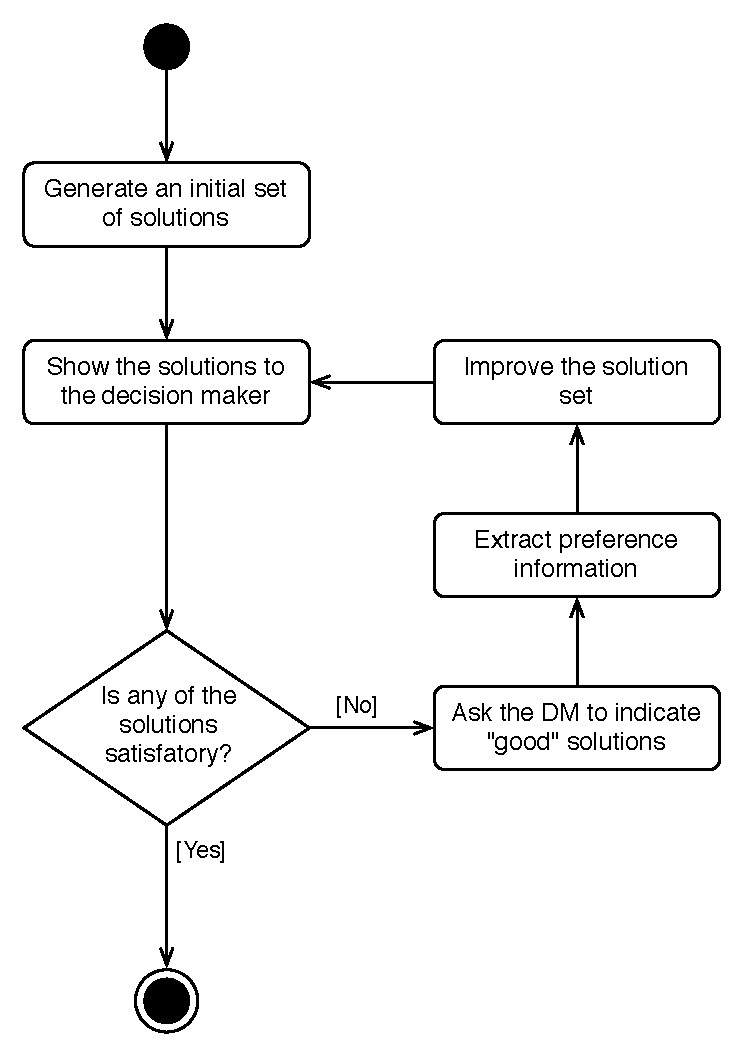
\includegraphics[scale=0.65]{img/imoprocess_uml}
  \caption{An activity diagram for a typical interactive process}
  \label{imoprocess_uml}
\end{figure}

From the DM's answers a preference model is built. This additional preference
information guides the search towards a~region indicated by the Decision
Maker. This can save the computational cost, because the algorithm doesn't
have to go through the whole search space.

Again, new solutions, probably better fitted to the DM's preferences are
generated and the algorithm shows them to he or she. If he or she finds it
satisfactory (or a~stop condition is met) then the algorithm stops. Otherwise
it advances to the next iteration.

There are several types of the IMO methods (consult~\cite{MRW08} for an
in-depth description):
\begin{itemize}
\item \textbf{Trade-off based methods}. A~trade-off is an exchange, a price that
  one is willing to pay (in form of lost on some of the criteria), in order to
  benefit on another criterion (or criteria). These methods ask the DM
  questions about the trade-offs he or she can accept and then, a~preference
  model is inferred based on the tread-offs.
\item \textbf{Reference point approaches} where the DM specifies bounds on
  values of the objective functions (i.e. reference points) and can observe
  the effect of this points on the generated solutions.
\item \textbf{Classification-based methods}. It is not possible to improve a
  value of a goal of a solution from the Pareto-frontier without worsening
  another goals of the solutions. In the classification-based methods the DM
  is asked to select goals that can be impaired and the ones that he or she
  wants to improve.
\end{itemize}

The interactive approach requires the Decision Maker's collaboration during
the process, however it has strong benefits to justify this
dedication. Clearly, the computational cost required is lower than in other
approaches, because there is no need to evaluate whole solution space, just
its small subset. The DM may not be able to express global structure of his or
her preferences up front. It is also possible that his or her preferences will
change along with the change in problem understanding. During the interactive
process the DM has an immediate feedback --- he or she may see how the
decisions are affecting problem solutions.

One can say that solving a Multi-Objective Optimization problem is a
constrictive process, where the Decision Maker learns more about the problem
--- what kind of solutions are possible and how his of her choices influences
the results (see~\cite{MRW08}). As a result, not only the most preferred
solution is given, but also the problem understanding by the DM is better.


\section{Evolutionary Approaches to MOO}
\label{sec_ea_in_moo}


\section{Dominance-Based Rough Set Approach in MOO}
\label{sec_drsa_in_moo}


%%% Local Variables: 
%%% mode: latex
%%% TeX-master: "main"
%%% End: 
